\documentclass{article}
\usepackage{graphicx} % Required for inserting images
\usepackage{caption} % Required for \captionof
\usepackage{amsmath}
\usepackage{float}
\usepackage{comment}
\usepackage[T1]{fontenc}
\usepackage[utf8]{inputenc}
\usepackage{lmodern}
\usepackage{microtype}
\usepackage{xcolor}
\usepackage{framed}
\renewenvironment{leftbar}{%
  \def\FrameCommand{\textcolor{orange}{\vrule width 3pt} \hspace{10pt}}%
  \MakeFramed {\advance\hsize-\width \FrameRestore}}%
 {\endMakeFramed}

\title{Hőtani mérés}
\author{Kern Luca, Csongor Vincze}
\date{2026 Április 14}

\begin{document}

\maketitle

\section*{5. Feladat: Határozza meg egy inhomogén tömegeloszlású lemezből készült minta tehetetlenségi nyomatékát a súlypontján átmenő és a lemez síkjára merőleges tengelyre vonatkozóan!}

\[
T'^2_{\max} = \frac{4\pi^2}{k^*} \left[ \theta + \theta_x + m(r_0 + r_1)^2 \right],
\]

\[
T'^2_{\min} = \frac{4\pi^2}{k^*} \left[ \theta + \theta_x + m(r_0 - r_1)^2 \right],
\]

%fotó, minta!!!!

$m_{minta}= 0,387 \text{kg}$
A mintát úgy rögzítjük a 30°-os jelölésnél, hogy a csúcsnál lévő szöfelezővel essen egyvonalba az osztás.

$r_{1}= 5 \text{cm}$
Azért ezt a lyukat választottuk, mert ezt van a középponttól legtávolabb.

Hegyeszögnél lévő lyuknál rögzítettük:

\begin{table}[H]
    \centering
    \begin{tabular}{|c|c|}
        \hline
        Szögelfordulás [°] & 10 lengés lengési ideje [s] \\ \hline
         0 & 17,91 \\ \hline 
         30 & 17,71 \\ \hline
         60 & 16,99 \\ \hline 
         90 & 15,93 \\ \hline
         120 & 14,75 \\ \hline 
         150 & 14,03 \\ \hline
         180 & 13,66 \\ \hline
         210 & 13,99 \\ \hline
         240 & 14,60 \\ \hline
         270 & 15,88 \\ \hline
         300 & 16,77 \\ \hline
         330 & 17,58\\ \hline
        
    \end{tabular}
    \caption{Lengési idők az 5cm-nél lévő lyukkal, hegyesszög}
    \label{tab:lengesiido_1.1}
\end{table}

Tompa szögnél lévő lyuknál rögzítettük:

\begin{table}[H]
    \centering
    \begin{tabular}{|c|c|}
        \hline
        Szögelfordulás [°] & 10 lengés lengési ideje [s] \\ \hline
         0 & 16,63 \\ \hline 
         30 & 17,28 \\ \hline
         60 & 17,91\\ \hline 
         90 & 17,25 \\ \hline
         120 & 16,60 \\ \hline 
         150 & 15,59 \\ \hline
         180 & 14,59 \\ \hline
         210 & 14,06 \\ \hline
         240 & 13,99 \\ \hline
         270 & 14,18 \\ \hline
         300 & 15,07 \\ \hline
         330 & 15,93 \\ \hline
        
    \end{tabular}
    \caption{Lengési idők az 5cm-nél lévő lyukkal, tompaszög}
    \label{tab:lengesiido_1.2}
\end{table}

$r_{2}= 2 \text{cm}$
Azért ezta szöget választottuk, mert ez van a középponthoz legközelebb

Hegyesszögnél lévő furatnál rögzítve:

\begin{table}[H]
    \centering
    \begin{tabular}{|c|c|}
        \hline
        Szögelfordulás [°] & 10 lengés lengési ideje [s] \\ \hline
         0 & 15,09 \\ \hline 
         30 & 15,13 \\ \hline
         60 & 14,59\\ \hline 
         90 & 14,45\\ \hline
         120 & 13,84 \\ \hline 
         150 & 13,48 \\ \hline
         180 & 13,44 \\ \hline
         210 & 13,41 \\ \hline
         240 & 13,81 \\ \hline
         270 & 14,25 \\ \hline
         300 & 14,73 \\ \hline
         330 & 14,98 \\ \hline
        
    \end{tabular}
    \caption{Lengési idők az 2cm-nél lévő lyukkal, hegyesszög}
    \label{tab:lengesiido_2.1}
\end{table}

Tompaszögnél lévő luyknál rögzítve:

\begin{table}[H]
    \centering
    \begin{tabular}{|c|c|}
        \hline
        Szögelfordulás [°] & 10 lengés lengési ideje [s] \\ \hline
         0 & 14,47 \\ \hline 
         30 & 14,84 \\ \hline
         60 & 14,92 \\ \hline 
         90 & 14,72 \\ \hline
         120 & 14,33 \\ \hline 
         150 & 14,05 \\ \hline
         180 & 13,75 \\ \hline
         210 & 13,40 \\ \hline
         240 & 13,27 \\ \hline
         270 & 13,45 \\ \hline
         300 & 13,71 \\ \hline
         330 & 14,11\\ \hline
        
    \end{tabular}
    \caption{Lengési idők az 2cm-nél lévő lyukkal, tompaszög}
    \label{tab:lengesiido_2.2}
\end{table}

$r_{3}= 3 \text{cm}$

Hegyesszögnél lévő furatnál rögzítve:

\begin{table}[H]
    \centering
    \begin{tabular}{|c|c|}
        \hline
        Szögelfordulás [°] & 10 lengés lengési ideje [s] \\ \hline
         0 & 15,89 \\ \hline 
         30 & 15,62 \\ \hline
         60 & 15,41 \\ \hline 
        
    \end{tabular}
    \caption{Lengési idők a harmadik lyukkal}
    \label{tab:lengesiido_3.1}
\end{table}

Tompaszögnél lévő lyuknál rögzítve:



\begin{figure}[H]
    \centering
    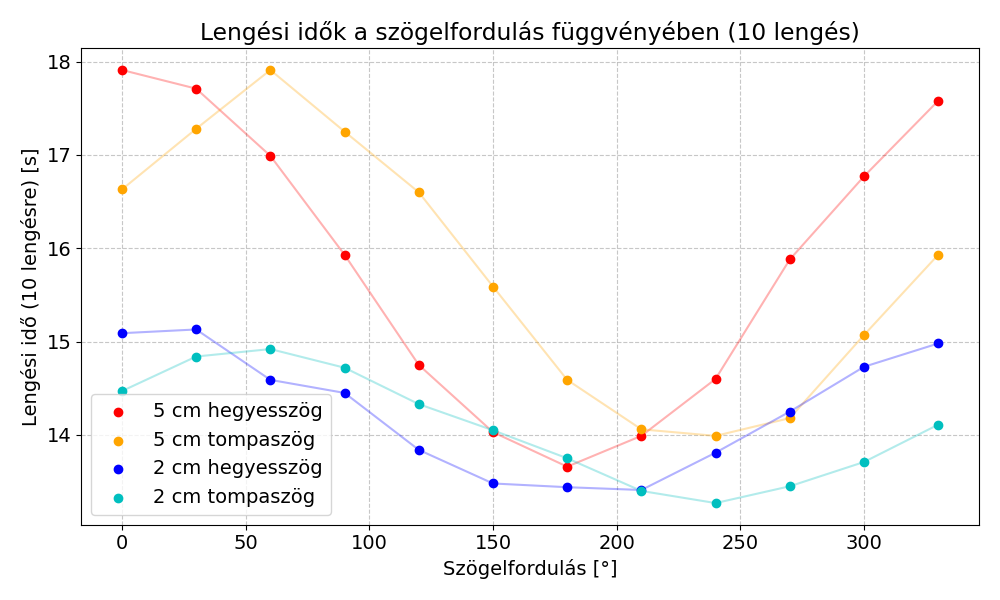
\includegraphics[width=0.8\textwidth]{../images/5_feladat.png}
    \caption{Mérési adatok, az azonos mérésehez tartozóak halványan összekötve}
    \label{fig:4}
\end{figure}

A tehetetlenségi noymaték kiszámítására nem maradt időnk. Az időhiány miatt amúgy se maradt időnk az összes lehetséges rögzítési pontnál megmérni a lengési időket, de a középponthoz legközelebbi, és attól legtávolabbi pontban megmértük. Egy harmadik pontotban is elkezdtünk mérni, de nem maradt időnk befejezni.


\end{document}